\documentclass[a4paper, 12pt]{extbook}

% inserire il conteggio fino alle subsubsection
\setcounter{secnumdepth}{3}

% Stile delle intestazioni
\usepackage{fancyhdr}
\pagestyle{fancy}
\fancyhf{} % Svuota le intestazioni e i piè di pagina
\fancyhead[LE,RO]{} % Rimuove il titolo del capitolo dalle intestazioni
\fancyfoot[C]{\thepage} % Mantiene il numero di pagina al centro del piè di pagina

\pagestyle{plain}

% Packages
\usepackage[utf8]{inputenc}
\usepackage[T1]{fontenc}
\usepackage{lmodern}
\usepackage[italian]{babel}
\usepackage{hyperref}
\usepackage{geometry}
\geometry{a4paper, margin=1in}
\usepackage{graphicx}
\usepackage{listings}
\usepackage{xcolor} 
\usepackage{booktabs} % Per linee migliori nelle tabelle
\usepackage{multirow} % Per più funzionalità nelle tabelle

% Title Page Information
\title{
    
\includegraphics[width=0.4\textwidth]{img/logo_unina.png} \\ % Modifica 'logo' con il nome del file del tuo logo
    \vspace{1cm}
    \Large{Appunti di\\}
    \Huge{Architettura e progettazione dei calcolatori} \\
    \vspace{0.5cm} 
    \Large{Corso di laurea magistrale in} \\
    \Large{\textbf{Ingegneria Informatica}}
}
\author{\textbf{}} % Modifica con il tuo nome
\date{}

% Motorola 68k sensitive
\lstdefinelanguage{Motorola68k}{
    morekeywords={MOVE, ADD, SUB, MULS, MULU, DIVS, DIVU, AND, OR, EOR, NOT, CLR, NEG, EXT, CMP, TST, BSET, BCLR, BCHG, BTST, BRA, BSR, BEQ, BNE, BCC, BCS, BVC, BVS, BPL, BMI, BGE, BLT, BGT, BLE, DBEQ, DBNE, DBCC, DBCS, DBVC, DBVS, DBPL, DBMI, DBGE, DBLT, DBGT, DBLE, JMP, JSR, RTS, RTE, RTD, TRAP, STOP, RESET, NOP, LEA, PEA, LINK, UNLK, SWAP, EXG, EXT, ASL, ASR, LSL, LSR, ROL, ROR, ROXL, ROXR, ADDA, ADDQ, SUBA, SUBQ, BLS, BHI, CMPI, CMPA, TAS, MOVEA, MOVEM, ORG, DS, DC, EQU, ANDI},
    morecomment=[l]*,
    morecomment=[n]{/*}{*/},
    morestring=[b]\",
    morestring=[b]',
    sensitive=true,
    keywordstyle=\bfseries\color{blue},
    commentstyle=\itshape\color{gray},
    stringstyle=\color{red},
    basicstyle=\ttfamily\small,
}

\lstset{
  language=Motorola68k,
  basicstyle=\ttfamily\small, % Font del codice
  keywordstyle=\color{blue}\bfseries, % Stile delle keyword
  commentstyle=\color{green!50!black}\itshape, % Stile dei commenti
  stringstyle=\color{red}, % Stile delle stringhe
  numbers=left, % Numeri di linea a sinistra
  numberstyle=\tiny, % Font dei numeri di linea
  stepnumber=1, % Intervallo delle linee numerate
  breaklines=true, % Spezza automaticamente le righe lunghe
  frame=single, % Bordo intorno al codice
  rulecolor=\color{gray}, % Colore del bordo
  backgroundcolor=\color{gray!10}, % Colore di sfondo
  tabsize=2, % Ampiezza del tab
  captionpos=b, % Posizione della didascalia
  showstringspaces=false % Non mostra gli spazi nelle stringhe
}

% Document
\begin{document}

% Title Page
\maketitle
\newpage

% Table of Contents
\tableofcontents
\newpage

% Include chapters
\chapter*{Introduzione}
\addcontentsline{toc}{chapter}{Introduzione}
FNS

\chapter{Richiami ed approfondimenti sui sistemi di
elaborazione}
In questo capitolo sarà affrontata principalmente la parte iniziale del corso che si occupa della scrittura di programmi utilizzando il linguaggio Motorola 68k. L'interesse non sarà volto alla tipologia di architettura, anche se a volte ci sarà il bisogno di specificarla, quanto al suo utilizzo effettivo nell'ambito del corso

 \section{Richiami di calcolatori elettronici}
Il Motorola 68k è un microprocessore con architettura di tipo CISC, essa è principalmente costituita da vari registri con diverse tipologie di utilizzo. Tali registri, però, non sono una caratteristica specifica dell'architettura del Motorola 68k, pertanto è buona norma introdurre l'architettura generale di vari tipologie di microprocessori. Tali caratteristiche, quindi, non sono intrinseche del solo Motorola 68k ma sono legate alla natura stessa delle varie microarchitetture dei vari processori.

\subsection{Architettura generale}
Quando si interagisce con le microarchitetture si lavora con vari tipologie di registri, la cui dimensione è descritta del costruttore.
I registri possono essere divisi principalmente in registri utilizzabili dal programmatore (o registri utilizzabili) e quelli che non possono essere utilizzati dal programmatore (o non utilizzabili). Tale suddivisione vi è poichè alcuni registri all'interno della microarchitettura vengono utilizzati per effettuare delle operazioni pilotate dalla CU. Tali registri sono tutti interni alla CPU (Ricordando che la cpu è formata da CU, ALU e registri interni). I registri interni utilizzabili dal programmatore sono anche chiamati \textbf{registri macchina (o registri general-purpose)} e possono essere di vario tipo:

\begin{itemize}
    \item \textbf{Registri Dato}: Registri che sono utilizzati per conservare un determinato dato su cui vado ad operare con varie tipologie di interazioni
    \item \textbf{Registri indirizzo}: Registri che sono utilizzati per conservare gli indirizzi a cui magari si vuole accedere in memoria (tipo puntatori in C/C++)
    \item \textbf{Registri Speciali}: Registri utilizzabili dal programmatore ma con funzioni diverse, ovvero:
    \begin{itemize}
        \item \textbf{PC (Program Counter)}: memorizza la posizione del prossimo comando da eseguire del nostro programma
        \item \textbf{IR (Istruction Register)}: Contiene una copia dell'istruzione prelevata dalla memoria
        \item \textbf{SR(Status Register)}: registro di stato che contiene varie tipologie di informazione, come il caso di overflow, di azzeramento del risultato, di grado di esecusione (se in administrator mode e quindi con l'accesso ad A'7)
    \end{itemize}
\end{itemize}

Tra i registri a cui invece il programmatore non ha accesso vi sono:
\begin{itemize}
    \item \textbf{MA (Memory Access)}: Registro utilizzato dal processore per scrivere l'indirizzo di memoria a cui si vuole accedere
    \item \textbf{MB (Memory Buffer)}: Registro che contiene il dato che si è letto/scritto in memoria (varia in base ai valori dei segnali di write e di read gestiti dalla CU)
\end{itemize}

\subsubsection{Memoria}
La memoria per noi funziona come un blocco a cui dati indicizzati. Per cui in base all'operazione che la CU va ad effettuare, modifica i valori di: MA, MB, segnale di read e di write.
Posso memorizzare i dati i memoria in vario modo, quindi posizionandoli in vario modo, tali posizioni rispettano le seguenti due tipologie di organizzazione:
\begin{itemize}
    \item \textbf{little-endian}: nella memorizzazione di un dato binario, riorganizzato in celle lunghe dei byte, i valori più significativi vengono memorizzati nelle celle con indirizzi più alti, mentre le meno significative in quelli con indirizzi più bassi
    \item \textbf{big-endian}: nella memorizzazione di un dato binario, riorganizzato in celle lunghe 1 Byte, esso sarà memorizzato inserendo i bit più significativi nelle celle con indirizzo più basso mentre i bit meno significativi in quelle con indirizzo più alto
\end{itemize}

\MakeUppercase{è} indifferente ai fini del funzionamento del processore quale sia la tipologia di organizzazione dei dati in memoria. Ma bisogna averne una conoscenza perchè è importante far capire all'unità di controllo come deve trattare i dati che sta andando a prelevare. Nel caso del Motorola 68k ci troviamo a contatto con un processore con organizzazione big-endian.
\\
Oltre all'organizzazione dei dati un altro problema della gestione della memoria è il suo allineamento in memoria, dato dal fatto della gestione delle sue celle di byte in maniera "indipendente".
Nel caso del motorola 68k, sono consentiti gli accessi in memoria anche a porzioni diverse di byte, ma tali porzioni hanno il vincolo di poter essere obbligatoriamente o da 2 o da 4 Byte che iniziano in posizioni di memoria pari. Quindi si possono avere degli errori se si accede a posizioni di memoria dispari
\\
A volte quando si lavora con gli indirizzi di memoria si può andare anche in contro al problema dell'\textbf{aliasing}, ovvero un problema che riguarda l'accesso a locazioni di memoria sbagliate rispetto a quelle effettivamente desiderate (nel caso del 68k questo problema è dovuto al fatto che possiede 24 fili di bus ma i registri sono a 32 bit, per cui se prelevo un indirizzo dalla memoria, perdendo gli 8 bit più significativi, se faccio accesso all'indirizzo caricato, posso confonderlo con uno più piccolo)
\\
\\
La memoria, quindi memorizza varie tipologie di dati e di istruzioni. Pertanto è corretto dividere la memoria rispetto a queste due parti, per cui, la memoria sarà organizzata da due principali parti:

\begin{itemize}
    \item \textbf{Area codice (o area istruzioni)}: Area dove sono contenuti i programmi e le istruzioni da eseguire
    \item \textbf{Area dati}: Area dove sono memorizzati i dati
\end{itemize}

In generale le aree minori sono le aree codice, mentre le restanti sono aree dati

\subsection{Istruzioni}\label{par:istruzioni}
In generale le istruzioni offerte dalle architetture, sono formate da tre principali parti:
\begin{itemize}
    \item \textbf{Codici operativi}: Operazioni elementari implementate in base all'architettura del processore, quindi istruzioni appartenenti al processore che specificano tutti i registri ed i passaggi da effettuare per determinate operazioni

    \item \textbf{Operandi sorgente}: Valori che possono essere memorizzati sia in dei registri interni che esterni (in base alla tipologia di operazione), su cui poi i codici operativi appartenenti all'istruzione vanno a lavorare

    \item \textbf{Operandi destinazione}: Registri o locazioni di memoria in cui si va ad inserire il dato prodotto dai codici operativi in base agli operandi sorgente ricevuti. Solitamente tale operando è indiretto poichè potrebbe diventare uno dei due operandi sorgente
\end{itemize}

In generale un istruzione è una composizione di bit, essa stessa immagazzinata in memoria, in cui una parte identifica il \textbf{codice operativo} da effettuare, mentre l'altra specifica gli operandi, che nel caso di registri interni vengono identificati con il corrispettivo indirizzo, mentre nel caso di indirizzi esterni viene specificata la locazione di memoria da cui prelevare il dato. Le tipologie di indirizzamento che posso essere utilizzate per gli operandi sono:
\begin{itemize}
    \item \textbf{Diretto}: Gli operandi presenti in memoria vengono acceduti specificando l'indirizzo di memoria in maniera plane
    \item \textbf{Indiretto}: Gli operandi in memoria vengono acceduti in base al valore puntato da un registro indirizzo
    \item \textbf{Implicito}: alcuni operandi sono dichiarati in maniera implicita all'interno dell'operando (Es. PUSH D3, pusha il valore in cima allo stack)
    \item \textbf{Immediato}: il dato da inserire in una determinata destinazione è direttamente inserito all'interno dell'istruzione (es. MOV \#7,D0)
    \item \textbf{Spiazzamento}: la locazione di memoria a cui si vuole fare riferimento viene acceduta tramite uno spiazzamento rispetto ad un indirizzo di memoria
    \item \textbf{Indice + spiazzamento}: la locazione di memoria a cui si vuole fare riferimento viene acceduta tramite un indice, che identifica una determinata zona della memoria rispetto ad un indirizzo (quindi tipo spiazzamento fisso) + un possibile ulteriore spiazzamento (per capire bene immaginarsi la memorizzazione e l'accesso a valori di una matrice)
\end{itemize}

% Da sistemare questa parte
Le istruzioni che vengono implementate per una particolare architettura vengono chiamate \textbf{ISA(Istruction Set Architecture)}, e che quindi possono essere o di tipo RISC o di tipo CISC in base alle scelte di progettazione.

Le architetture con cui sono progettate i più moderni processori possono essere di 2 tipologie:
\begin{itemize}
    \item \textbf{CISC (Complex-Istruction-Set-Computer)}: dove le istruzioni a disposizione del programmatore possono essere anche più complesse (comprendono l'utilizzo anche di più istruzioni semplici), un classico esempio è la memorizzazione di un dato in una memoria, che nel caso CISC può essere effettuato tramite un singolo comando

    \item \textbf{RISC (Reduced-Istruction-Set-Computer)}: L'architettura del microprocessore permette l'utilizzo di un set più ridotto di istruzioni, semplici e lineari, tali istruzioni a differenza del paradigma CISC, possono essere più veloci, ma non ripagano in termini di complessità per l'effettuazione di determinate operazioni (come nel caso della memorizzazione di una dato in memoria)
\end{itemize}

Nel nostro caso noi utilizzeremo il Motorola 68k a 16/32 bit, dove tali bit indicano la grandezza dei registri, e di conseguenza, dei bus di collegamento tra essi. L'architettura di tale microprocessore è CISC, ma noi utilizzeremo un set ridotto di tutte le funzioni messe a disposizione dall'M68k, in modo da poter avere anche la confidenza giusta per affrontare, in futuro, anche tipologie di architetture RISC.

Per l'esecuzione di una particolare istruzione, il microprocessore deve, prima prelevarla dalla memoria. La specifica su quale istruzione prelevare la conserva il PC (Program Counter) che conserva l'indirizzo di memoria da cui prelevare la prossima istruzione. Una volta prelevata l'istruzione dalla memoria tramite gli indirizzi MA ed MB, questa viene caricata nell'IR, che conserverà tale istruzione durante tutto il processo di decodifica ed esecuzione delle operazioni specificate

Le istruzioni, in generale possono essere classificate nel seguente modo:

\begin{itemize}
    \item \textbf{Trasferimento dati}: Codici che mi permettono di copiare un dato da un determinato operando e spostarlo nell'altro (MOVE)

    \item \textbf{Aritmetiche}: effettua delle operazioni aritmetiche sugli operandi in ingresso e le memorizza in un operando destinazione. Solitamente le funzioni appartenenti a tale classe lavorano su numeri interi

    \item \textbf{Logiche}: Operazioni che vengono effettuate sulle stringhe degli operandi con una logica bit a bit, effettuata l'operazione il risultato viene inserito all'interno di una data destinazione

    \item \textbf{Scorrimento}: operazioni effetuate sugli operandi in ingresso che restituiscono lo scorrimento verso (destra o sinistra) dell'operando e lo memorizzano in una data destinazione

    \item \textbf{Confronto}: gli operandi vengono confrontati ed in base alla tipologia di controllo che voglio effettuare vado a controllare i valori dell'SR che mi interessano

    \item \textbf{Salto}: Le istruzioni di salto permettono di cambiare il PC e quindi di eseguire (o rieseguire) delle porzioni di codice a cui puntano. Le istruzioni di salto possono essere di tipo condizionato(Bcc) o non condizionato (JMP). Nel primo caso l'istruzione di salto viene effettuata solo se è vera una data condizione, mentre nel secondo caso il salto viene effettuato senza il controllo di alcuna condizione

    \item \textbf{Input/Output}: Alcune CPU sono dotate di apposite istruzioni per trasferire i dati da e verso le periferiche apposite
\end{itemize}

\section{Motorola 68k}
Una volta introdotti i concetti teorici e tecnologici propedeutici, si possono iniziare ad osservare i principali costrutti per la programmazione con il Motorola 68000.
Conviene, quindi, non solo capire quali sono i  codici per le varie tipologie di istruzioni specificate nel paragrafo [\ref{par:istruzioni}], ma anche come costruire i principali componenti di un linguaggio di più alto livello (di cui si presuppone una minima conoscenza). I costrutti in questione possono essere: cicli, blocchi di decisione, ecc.

\subsection{Registri General Purpose}
Con \textit{registri General-Purpose} (o registri macchina) intendiamo l'insieme dei registri messi a disposizione del programmatore per scrivere codice sfruttando i codici operativi dell'ISA.
I registri General-Purpose a disposizione sono un insieme di registri a 32 bit:
\begin{itemize}
    \item \textbf{Registri Dato}: Registri D0,D1,\dots,D7;
    \item \textbf{Registri Indirizzo}: Registri A0,A1,\dots,A7 ed A7' (questi ultimi puntano alla cima dello STACK: A7' è accessibile solo in modalità \textit{supervisore}. In generale, ogni modalità di esecuzione dispone di un'area stack separata);
    \item \textbf{Status Register (SR)}: Registro a 16 bit che contiene informazioni sia sui risultati delle operazioni dell'ALU che sullo stato dell'esecuzione (se in super-user o meno). Questo regsitro è sempre accessibile in lettura, mentre è accessibile in scrittura solo in modalità supervisore.
\end{itemize}

\begin{table}[h!]
\centering
\renewcommand{\arraystretch}{1.2}
\begin{tabular}{|c|c|c|}
\hline
\textbf{Bit} & \textbf{Sigla} & \textbf{Descrizione} \\
\hline
15 & T & Trace Enable \\
\hline
14 & S & Supervisor State (1=Supervisor) \\
\hline
13-8 & - & Non usati (riservati) \\
\hline
7 & X & Extend (Estensione del Carry) \\
\hline
6 & N & Negative \\
\hline
5 & Z & Zero \\
\hline
4 & V & Overflow \\
\hline
3 & C & Carry \\
\hline
2-0 & - & Non usati (riservati) \\
\hline
\end{tabular}
\caption{Bit dello Status Register (SR) del Motorola 68k}
\label{table:SR68k}
\end{table}


\subsection{Codici di Spostamento dati o indirizzi}
Il principale codice operativo che nel motorola 68k permette lo spostamento dei dati è la \lstinline|MOVE|, che può essere differentemente utilizzata in base ai seguenti parametri:

\begin{itemize}
    \item \textbf{Lunghezza degli operandi}: solitamente specificata con la \textit{dot notation} alla fine del comando;
    \item \textbf{Tipologia di indirizzamento}: La \lstinline|MOVE| è una tra le poche operazioni che ammette tutte le tipologie di indirizzamento possibili (proprietà detta di \textbf{ortogonalità}); L'indirizzamento immediato per l'operando di destinazione è l'unico che può causa errore, ma è un'operazione che comunque non ha alcun senso.
\end{itemize}

La caratterizzazione del comando \lstinline|MOVE| è la seguente:
\begin{lstlisting}
    *Indirizzamento diretto D1 = D0 o D1<-D0
    MOVE D0,D1

    *Indirizzamento indiretto (sorgente), diretto (destinazione)
    *D0 = (A0), D0 = contenuto del registro in posizione A0
    MOVE.W (A0),D0

    *Indirizzamento Indiretto completo
    MOVE.L (A0),(A1) *(istruzione non valida)
    *o
    MOVEA.L (A0),A1 *(istruzione valida)
    *Indirizzamento immediato + indirizzamento Diretto
    MOVE.L #14,D0

    * Indirizzamento con spiazzamento su registro di indirizzo
    MOVE.W 4(A0), D0    * D0 = valore all'indirizzo A0 + 4

    * Indirizzamento con spiazzamento e registro indice
    MOVE.L 8(A0, D1.L), D2   * D2 = valore all'indirizzo A0 + 8 + D1

    * Indirizzamento PC relativo con spiazzamento
    MOVE.B 6(PC), D0   * D0 = byte situato 6 byte dopo il Program Counter

    * Push di un registro nello Stack
    MOVE.L D0, -(A7)   * Salva D0 nello stack (decremento SP)

    * Pop dallo Stack in un registro
    MOVE.L (A7)+, D0   * Carica D0 con il valore in cima allo stack (incremento SP)

    * Push di un registro di indirizzo
    MOVEA.L A0, -(A7)  * Salva A0 nello stack

    * Pop di un registro di indirizzo
    MOVEA.L (A7)+, A0  * Carica A0 con il valore in cima allo stack

    * Salvataggio multiplo nello stack
    MOVEM.L D0-D3/A0-A2, -(A7)  * Salva piu' registri nello stack

    * Ripristino multiplo dallo stack
    MOVEM.L (A7)+, D0-D3/A0-A2  * Ripristina piu' registri dallo stack

    * Ritorno da subroutine (equivalente a POP del PC)
    RTS   * Ritorna dall'ultima subroutine chiamata
\end{lstlisting}

\textbf{Nota sull'indirizzamento indiretto completo}: Non è possibile utilizzare un'operazione del tipo \lstinline|MOVE (A0), (A1)| perchè il bus dati dell'architettura del MC68k non supporta simultaneamente operazioni di lettura e scrittura, dunque servono due cicli di bus distinti. Occorre utilizzare dei registri dato interni di appoggio.

\textbf{Nota su} \lstinline|MOVE.L D0, -(A7)|: il pre-decremento nell'operazione di push nello stack è dovuto al fatto che, per costruzione, lo stack "cresce" verso il basso, quindi deve decrescere di 4 byte per ospitare quanto vi sto inserendo (quanto detto è scollegato dal fatto che il 68k sia big endian).

\textbf{Nota su RTS}: come concetto, RTS equivale a MOVE.L (A7)+, PC perché il valore puntato da A7 è quello * in cima allo stack, in questo caso estraiamo quindi + (lo stack "sale"), in caso contrario avremmo avuto - (quando inseriamo nello stack).

Nel codice precedente sono da notare le seguenti notazioni:
\begin{itemize}
    \item \textbf{.W}: tale parte del comando permette di capire che sto lavorando con operandi lunghi 16 bit (o 2 Byte) esse sono denotate Word. Nel caso in cui non sia specificato alcun markup, allora la move è da intendersi per soli 8 bit
    \item \textbf{.L}: tale parte del comando permette di capire che sto lavorando con operandi lunghi 32 bit (o 4 Byte) esse sono denotate Long Word
    \item \textbf{\#14}: Vado ad identificare un valore immediato tramite il termine \#<valore>, che sarà convertito in binario dal compilatore e poi inserito all'interno del programma, quindi integrato all'interno della zona istruzioni della mia memoria
\end{itemize}

\newpage

\subsection{Codici Aritmetici}
Per il motorola vi sono vari codici aritmetici, che però possono lavorare solo su valori interi e quindi non valori "reali" (o codificati in IEEE 754).
I codici aritmetici più importanti, ed in generale, più presenti all'interno delle varie architetture sono i seguenti:

\subsubsection{Somma}

\begin{lstlisting}
    *Operatore di somma
    ADD #3, D0  *immediato + diretto, D0 = 3+D0
    ADD.W #3,D0 *somma con specifica grandezza valore D0 = 3+D0
    ADD.W D0,D1 *indirizzamenti diretti con D1 = D0+D1

    ADDA.L #1,A0 *somma su registri di tipo indirizzo, somma 1 direttamente al contenuto di A0, non alla locazione di memoria puntata da A0 (NON ci sonon le parentesi)

    ADDQ.W #1,D0 *somma di un valore immediato tra 1 e 8
\end{lstlisting}

\subsubsection{Sottrazione}

\begin{lstlisting}
    *Operatore di Sottrazione
    SUB #3, D0  *immediato + diretto, D0=D0-3
    SUB.W #3,D0 *sotterazione con specifica grandezza valore D0=D0-3
    SUB.W D0,D1 *indirizzamenti diretti con D1=D1-D0

    SUBA.L #1,A0 *Sottrazione su registri di tipo indirizzo

    SUBQ.W #1,D0 *Sottrazione di un valore immediato tra 1 e 8
\end{lstlisting}

\subsubsection{Moltiplicazione}

\begin{lstlisting}
    MULU #3, D0      * Moltiplicazione senza segno immediato + diretto, D0 = D0 * 3
    MULU.W #3,D0     * Moltiplicazione senza segno con specifica grandezza valore, D0 = D0 * 3
    MULU.W D0,D1     * Moltiplicazione senza segno con indirizzamento diretto, D1 = D1 * D0

    MULS.W #3,D0     * Moltiplicazione con segno immediato + diretto, D0 = D0 * 3
    MULS.W D0,D1     * Moltiplicazione con segno tra registri, D1 = D1 * D0
\end{lstlisting}

\subsubsection{Divisione}

\begin{lstlisting}
    DIVU #3, D0      * Divisione senza segno immediato + diretto, D0 = D0 / 3 (quoziente in D0, resto in D1)
    DIVU.W #3,D0     * Divisione senza segno con specifica grandezza valore, D0 = D0 / 3
    DIVU.W D0,D1     * Divisione senza segno con indirizzamento diretto, D1 = D1 / D0

    DIVS.W #3,D0     * Divisione con segno immediato + diretto, D0 = D0 / 3
    DIVS.W D0,D1     * Divisione con segno tra registri, D1 = D1 / D0
\end{lstlisting}

Come si nota dalle varie implementazioni dei codici aritmetici, questi non possono utilizzare tipologie di indirizzamento indiretto. Pertanto, prima di effettuare le operazioni aritmetiche, gli operandi di input devono essere caricati nei registri interni ed il risultato sarà poi memorizzato in uno dei due registri impiegati (Come visibile nei commenti dei vari comandi).
Inoltre, sia MULU e MULS che DIVU e DIVS lavorano implicitamente su 16 bit nel 68k, e non esistono cose del tipo MULU.B oppure MULU.L (idem per gli altri 3 codici operativi).

\subsection{Codici di salto} \label{par:salto}

I codici di salto possono essere di 3 tipologie principali nel motorola 68k:
\begin{itemize}
    \item \textbf{Salti incondizionati}: Quando viene incontrata l'istruzione di salto, questa effettua il salto (cambiamento del PC) in maniera immediata e senza la verifica di alcuna condizione;

    \item \textbf{Salti condizionati}: I salti condizionati sono effettuati in base al verificarsi di una determinata condizione. Nel caso del motorola 68k la condizione è associata ai valori dei singoli bit dello Statur Register (SR);

    \item \textbf{Salti a subrutine}: I salti a subroutine sono delle tipologie particolari di salto incondizionato, con l'unica differenza che l'indirizzo di memoria da cui si è saltati viene prima memorizzato nello stack e poi viene effettuato il salto. Tale operazione fa in modo che una volta eseguita la subroutine, il sistema possa ritornare al punto a cui si era fermato nel programma principale, sollevando il programmatore dall'onere di gestire manualmente il salvataggio dell'indirizzo di ritorno.
\end{itemize}

In generale, quando si definisce un codice di salto, bisogna prevedere anche il suo operando, che dal lato del programmatore può essere di principalmente 2 tipi:
\begin{itemize}
    \item \textbf{Label}: dopo l'istruzione si fa riferimento ad una label all'interno del programma scritto che permette di evitare di andare a lavorare con indirizzi di memoria diretti (sarà il compilatore a configurarli ad-hoc);

    \item \textbf{Indirizzamento indiretto}: Tramite dei registri indirizzo si indica la locazione di memoria specifica a cui si vuole saltare;
\end{itemize}

\newpage
\subsubsection{Salti non condizionati}
I salti non condizionati in motorola possono essere i seguenti:
\begin{lstlisting}
    BRA label      * Salto incondizionato alla label specificata (branch always)
    JMP address    * Salto incondizionato all'indirizzo specificato
    JMP (A0)       * Salto all'indirizzo contenuto in A0
\end{lstlisting}

Solitamente nelle varie applicazioni si preferisce utilizzare il comando BRA, poichè più semplice da ricordare in riferimento ai comandi di salto condizionato.

\subsubsection{Salti condizionati}
I salti condizionati hanno una forma più o meno uguale in base a quello che si vuole fare. La loro forma nel caso del 68k è del tipo: Bcc. Dove la B sta per BRANCH mentre "cc" sono le componenti che permettono di distinguere la condizione da considerare rispetto ai valori dello SR. In particolare, i salti condizionati operano in base ai valori dei 5 bit del \textbf{CCR (Condition Code Register)}, che sono i 5 bit meno significativi dello SR riportati in tabella \ref{table:SR68k}.

I principali comandi sono i seguenti:
\begin{lstlisting}
    BCS label      * Salto se Carry e' settato (C = 1)
    BCC label      * Salto se Carry e' azzerato (C = 0)
    BVS label      * Salto se Overflow e' settato (V = 1)
    BVC label      * Salto se Overflow e' azzerato (V = 0)
    BEQ label      * Salto se Zero e' settato (Z = 1)
    BNE label      * Salto se Zero e' azzerato (Z = 0)
    BMI label      * Salto se Negativo e' settato (N = 1)
    BPL label      * Salto se Positivo e' settato (N = 0)

    BLT label      * Salto se Minore di (N XOR V = 1)
    BLE label      * Salto se Minore o uguale ((N XOR V) + Z = 1)
    BGT label      * Salto se Maggiore ((N XOR V) + Z = 0)
    BGE label      * Salto se Maggiore o uguale (N XOR V = 0)

    BLS label      * Salto se Minore o uguale (C + Z = 1) (senza segno)
    BHI label      * Salto se Maggiore (C + Z = 0) (senza segno)
\end{lstlisting}

\newpage

\subsubsection{Salti a subroutine}
I salti a subroutine sono una tipologia di salto incondizionato. Tali salti fanno parte di architetture CISC principalmente, poichè alcune architetture RISC non prevedono tali funzioni. La presenza di tali funzioni permette di non dover gestire l'indirizzo di ritorno dalla subroutine, o almeno non direttamente dal programmatore. Le istruzioni che in motorola 68k sono principalmente utilizzate per la chiamata a subroutine sono le seguenti:
\begin{lstlisting}
    * Salta a una subroutine e salva il ritorno nello stack 
    * (push nello stack)
    BSR label
    *Salta a una subroutine con indirizzo specifico o label
    JSR address/label
    * Ritorna dalla subroutine (estrae l'indirizzo di 
    * ritorno dallo stack, fa il pop dallo stack)
    RTS
\end{lstlisting}

\subsection{Codici Logici}
I codici logici sono operazioni che possono essere effettuate su degli operandi lavorando bit a bit. Da notare che per i codici logici si può avere l'indirizzamento indiretto solo per la sorgente e non per il destinatario. Esempi di codici logici sono i seguenti:
\begin{lstlisting}
    AND #3, D0      * AND bit a bit con valore immediato, D0=D0&3
    AND.W D0, D1    * AND tra registri, D1=D1&D0
    AND.L (A0), D0  * AND tra valore puntato da A0 e D0

    OR #3, D0       * OR bit a bit con valore immediato, D0=D0|3
    OR.W D0, D1     * OR tra registri, D1=D1|D0
    OR.L (A0), D0   * OR tra valore in memoria puntato da A0 e D0

    EOR #3, D0      * XOR bit a bit con valore immediato, D0=D0XOR3
    EOR.W D0, D1    * XOR tra registri, D1 = D1 XOR D0
    EOR.L (A0), D0  * XOR tra valore puntato da A0 e D0

    NOT D0          * Complemento bit a bit (negazione), D0 = ~D0
\end{lstlisting}

\newpage

\subsection{Codici di Scorrimento}
I codici di scorrimento permettono di effettuare delle operazioni di shift, che possono essere comode in alcune tipologie di operazioni
\begin{lstlisting}
    ASL #1, D0      * Shift aritmetico a sinistra di 1 bit 
                    *(mantiene il segno)
    ASR #1, D0      * Shift aritmetico a destra di 1 bit

    LSL #1, D0      * Shift logico a sinistra di 1 bit (0 fill)
    LSR #1, D0      * Shift logico a destra di 1 bit

    ROL #1, D0      * Rotazione a sinistra di 1 bit 
                    * (il bit piu' alto rientra da destra)
    ROR #1, D0      * Rotazione a destra di 1 bit

    ROXL #1, D0     * Rotazione a sinistra con Carry
    ROXR #1, D0     * Rotazione a destra con Carry
\end{lstlisting}

Osserviamo che lo shift aritmetico a sinistra ha l'effetto di moltiplicare per 2 (se convertiamo da decimale a binario il valore del registro prima e dopo lo shift), tranne se perdi bit significativi o alteri il segno, e dopo lo shift aritmetico possono essere modificati i bit del CCR.

\subsection{Codici di Confronto} \label{par:confronto}
I codici di confronto sono molto importanti, poiché in accoppiata con i salti condizionati permettono di costruire tutti i costrutti fondamentali che possiamo trovare anche nei linguaggi di alto livello
\begin{lstlisting}
    CMP #5,D0       * Confronta D0 con 5 (D0 - 5, senza 
                    * modificare D0, aggiorna i flag)
    CMP.W D0,D1     * Confronta D1 con D0 (D1 - D0, 
                    * aggiorna solo i flag)
    CMP.L (A0),D0   * Confronta D0 con il valore in 
                    * memoria puntato da A0
    CMPI #10,D0     * Confronto immediato con D0
                    * (D0 - 10, aggiorna solo i flag)
    CMPA.L #1000,A0 * Confronta registro indirizzo A0 con 1000
\end{lstlisting}

Oltre a semplici comparazioni, solitamente, vi sono anche dei comandi che operano sui singoli registri. Non solo per il controllo di tali registri ma anche per l'effettuazione di eventuali operazioni che possono essere comode per una tipologia di interpretazione ad alto livello del codice
\begin{lstlisting}
    TST D0          * Testa D0 (controlla se e' zero o negativo, 
                    * senza modificarlo)
    TST.W (A0)      * Testa il valore in memoria puntato da A0
    BTST #3, D0     * Testa il bit 3 di D0 
                    * (imposta Z se il bit e' 0)
    BTST #5, (A0)   * Testa il bit 5 della memoria puntata da A0
    BSET #3, D0     * Imposta il bit 3 di D0 a 1
    BSET #5, (A0)   * Imposta il bit 5 della memoria puntata da A0
    BCLR #3, D0     * Azzera il bit 3 di D0
    BCLR #5, (A0)   * Azzera il bit 5 del registro puntato da A0
    BCHG #3, D0     * Inverte il bit 3 di D0 (0 -> 1, 1 -> 0)
    BCHG #5, (A0)   * Inverte il bit 5 del registro puntato da A0
    TAS D0          * Testa e imposta il bit piu' alto (7) di D0
    TAS (A0)        * Testa e imposta il bit 7 del valore in 
                    * memoria puntato da A0
\end{lstlisting}

\subsection{Strutture sintattiche fondamentali}
Dati i codici di \textbf{Salto} [\ref{par:salto}] e quelli di \textbf{Confronto} [\ref{par:confronto}], si possono costruire quelle che sono le struttura sintattiche fondamentali

\subsubsection{if-then-else}
Per costruire il ciclo if-then-else bisogna per prima cosa comprendere quale sia la condizione, poichè bisognerà identificare:
\begin{itemize}
    \item \textbf{Registro target}: In base a quale registro/operazione devo decretare la condizione?
    \item \textbf{Condizione}: Qual'è la condizione da rispettare?
\end{itemize}

Scelti questi due parametri allora sarò capace di capire quale codice cmp utilizzare ed in che modo, e quale tipologia di salto condizionato effettuare.
Esempio di un classico If-Then:
\begin{lstlisting}
        MOVE.L  D0, D1  * Carica valori nei registri 
                        * (supponiamo che D0 e D1 abbiano   gia' valori)
        CMP.L   D1, D0  * Confronta D0 con D1 (D0 - D1)
        BGT     END_IF  * Se D0 > D1, salta al blocco then 
                        * (condizione = (D1 <= D0))
THEN                    * Codice interno all'IF
END_IF                  * Codice successivo...
\end{lstlisting}

Esempio di un If-Then-Else
\begin{lstlisting}
        MOVE.L  D0, D1  * Carica valori nei registri (supponiamo che D0 
                        * e D1 abbiano   gia' valori)
        CMP.L   D1, D0  * Confronta D0 con D1 (D0 - D1)
        BGT     THEN    * Se D0 > D1, salta al blocco THEN
ELSE    MOVE.L  #0, D2  * D2 = 0
        BRA     END_IF  * Salta oltre il blocco THEN 
THEN    MOVE.L  #1, D2  * D2 = 1
END                     * Codice successivo...
\end{lstlisting}


\subsubsection{Ciclo FOR}
Come per l'if il ciclo for è composto principalmente da codici di \textbf{salto} e da codici di \textbf{confronto}. La struttura è molto simile a quella dell'If-Then-Else con l'eccezzione della posizione dei vari salti.
Precisamente la struttura di un ciclo for è la seguente:
\begin{lstlisting}
    MOVE.L  #0, D0  * Inizializza il contatore D0 = 0

FOR CMP.L   #10, D0 * Confronta D0 con 10
    BGE     END     * Se D0 >= 10, esce dal ciclo

                    * Corpo del ciclo ...
    ADDQ.L  #1, D0  * Incrementa D0 di 1
    BRA     FOR     * Ripete il ciclo
END                 

\end{lstlisting}

\subsubsection{Ciclo While}

Il ciclo while segue le regole del ciclo for solo con una condizione differente:
\begin{lstlisting}
WHILE   CMP.L   #0, D1  * Confronta D1 con 0
        BLE     END     * Se D1 <= 0, esce dal ciclo
                        * Corpo del ciclo
        SUBQ.L  #1, D1  * Decrementa D1 di 1
        BRA     WHILE   * Ripete il ciclo
END                     * Codice successivo
\end{lstlisting}


\subsubsection{Chiamata a subroutine}

Le chiamate a subroutine possono essere viste come una sorta di chiamate a funzione. Esse, quindi, possono avere sia degli operandi di ingresso che degli operandi di uscita. La "comunicazione" degli operandi con la subroutine può avvenire in due principali modi:
\begin{itemize}
    \item \textbf{Con registri interni}: Gli operandi vengono caricati nei registri interni prima di chiamare la subroutine, che poi ci lavorerà sopra. Quindi i registri interni vengono utilizzati come una sorta di canale di comunicazione.
    \item \textbf{Con Stack}: Gli operandi sono allocati sullo stack, ciò richiede quindi una gestione anche del puntatore dello stack SP.
\end{itemize}

Un esempio di chiamata a subroutine con memorizzazione degli operandi nello stack è il seguente:
\begin{lstlisting}
        MOVE.L  #5, D0      * Carica il primo operando in D0
        MOVE.L  #10, D1     * Carica il secondo operando in D1
        MOVE.L  D0, -(A7)   * Push del primo operando nello stack
        MOVE.L  D1, -(A7)   * Push del secondo operando
        JSR     SUM_SUB     * Chiamata alla subroutine
        MOVE.L  (A7)+, D2   * prelievlo del risultato dallo stack
        ADDQ.L  #8, A7      * Pulizia dello stack 
                            * (2 valori da 4 byte)
                            * D2 ora contiene il risultato
                            * Codice successivo eventuale
SUM_SUB MOVE.L  (A7)+, D0   * Pop del primo operando dallo stack
        MOVE.L  (A7)+, D1   * Pop del secondo operando
        ADD.L   D1, D0      * Somma D0 + D1, risultato in D0
        MOVE.L  D0, -(A7)   * Push del risultato nello stack
        RTS                 * Ritorna al chiamante
\end{lstlisting}

Esempio di utilizzo dei registri interni, sia per passaggio operandi di ingresso che di uscita:

\begin{lstlisting}
        MOVE.L  #5, D0       * Primo operando in D0
        MOVE.L  #10, D1      * Secondo operando in D1

        JSR     SUM_REGS     * Chiamata alla subroutine
        * Dopo il ritorno, il risultato e' in D0
        * Codice successivo...
SUM_REGS:   ADD.L   D1, D0   * Somma D0 + D1, risultato in D0
        RTS                  * Ritorna al chiamante

\end{lstlisting}

\subsection{Valutazione degli accessi in memoria}
Utilizzando i comandi precedentemente presentati, il processore può accedere in memoria principale. Gli accessi in memoria dipendono fortemente dalla tipologia di architettura che ho adottato. In generale gli accessi in memoria possono avvenire per 2 tipologie di operazioni: Accesso in memoria per le Istruzioni (PI) o accesso in memoria Per le Operazioni (PO).
Veodiamo degli esempi per capire meglio di cosa si sta parlando:
\begin{table}[h]
    \centering
    \begin{tabular}{|c|c|c|}
        \hline
        \textbf{Istruzione} & \textbf{PI} & \textbf{PO} \\
        \hline
        \lstinline|MOVE.L D0,D1| & 1 & 0 \\
        \lstinline|MOVE.W D0,D1| & 1 & 0 \\
        \lstinline|MOVE.L #7,D1| & 3 & 0 \\
        \lstinline|MOVE.W (A0),(A1)| & 1 & 2 \\
        \lstinline|MOVE.W (A0),VAR| & 3 & 2 \\
        \hline
    \end{tabular}
    \caption{Conteggio accessi per Architettura a 16 bit e VAR a 32 bit}
    \label{tab:esempio}
\end{table}

Per contare gli accessi in memoria bisogna effettuare delle osservazioni in base alla parte che si sta analizzando.
Per l'accesso \textbf{Per le Istruzioni (PI)} si ragiona sui seguenti accessi:
\begin{itemize}
    \item \textbf{Prelievo dell'istruzione}: Un operazione che non mancherà mai sarà sempre il prelievo dell'istruzione, che impone che il mio PI non potrà mai essere nullo;
    \item \textbf{Operandi immediati}: se nel mio comando ho degli operandi immediati, allora dovrò accedere anche altre volte alla memoria per il prelievo di tale operando. I miei accessi, per questo caso, sono dettati dalla lunghezza dell'operando rispetto ai miei bus disponibili. Per esempio, se sono in un architettura a 16 bit devo prelevare un immegiato considerato una WORD, allora il numero di accessi aggiuntivi per prelevare l'immediato è uguale a 1. Mentre se stessi lavorango con le Long World (32 bit), allora il numero di accessi, a parità di architettura, sarà 2;
    \item \textbf{Variabili}: se sto utilizzando delle variabili, che indicano delle locazioni di memoria dirette, allora dovrò fare un numero di accessi alla memoria che mi permette di prelevare gli indirizzi (tali indirizzi sono lunghi tutti 32 bit). Pertanto con un architettura a 16 bit dovrò considerare sempre 2 accessi per ogni variabile per prelevare tali indirizzi;
\end{itemize}

Per l'accesso \textbf{Per gli Operandi (PO)}, i parametri risultano più o meno gli stessi, ad esclusione del prelievo istruzione e della variabile. Le operazioni che si contano per tale processo sono:
\begin{itemize}
    \item \textbf{Indirizzamento Indiretto}: quando vado ad effettuare dei riferimenti a dei registri della memoria con indirizzamento indiretto allora devo prevedere un numero di accessi per il prelievo dell'operando. Quindi bisogna conteggiare il numero di accessi per il prelievo dell'operando in base alla sua lunghezza. Nel caso di architettura a 16 bit si avranno: 1 accesso per prelevare delle word (16 bit) e 2 accessi pre prelevare le Long Word (32 bit)

    \item \textbf{Variabili}: Quando si utilizzano le variabili, oltre a prelevare gli indirizzi dalla "zona istruzioni" bisogna prelevare gli operando. La conta del numero di accessi per il prelievo degli operandi è uguale al caso di indirizzamento indiretto
\end{itemize}

Nel caso degli accessi PO, si è prevista la considerazione per singoli operandi. Quindi in base al numero di operandi presenti, la loro lunghezza prefissata, il loro modo di indirizzamento, si riesce a comprendere (cumulando le specifiche), il numero di accessi che bisogna effettuare in memoria ed il motivo di tali accessi.


 % Capitolo 1
\chapter{Gestione dei dispositivi di IO}
I dospositivi di input/output (o I/O), sono tutti quei dispositivi che si connettono alla classica architettura composta solo da processore e memoria centrale. Tra tali dispositivi rientrano: Memorie di massa (HDD e SSD), mouse, tastiera, sensori ecc.
Data l'eterogeneità di tali periferiche è richiesto che queste ultime siano gestite in un certo modo, o almeno, che la loro gestione principale sia di un certo tipo. Ciò, quindi, pone le basi su come dovremmo interfacciarci all'utilizzo di tali dispositivi

\section{Architettura generale di un dispositivo di I/O}
In generale un dispositivo di I/O può essere visto come l'insieme di tre parti fondamentali:
\begin{itemize}

    \item \textbf{Registri Dato, Stato e Controllo}: Tali registri sono quelli che interagiscono in maniera diretta con la CPU, e vengono utilizzati da quest'ultima per controllare e gestire le informazioni di quel dato dispositivo. Tali registri sono presenti internamente all'architattura del Calcolatore (ad esempio sulla scheda madre)

    \item \textbf{Sistema di adattamento}: Il sistema di adattamento adatta i segnali provenienti dal mondo esterno per essere letti o scritti nei registri di Dato, Stato e Controllo, e quindi permette di adattare l'attacco esterno (tipo l'USB che utilizza comunicazioni sequenziali), con la comunicazione parallela che il processore ha con i registri

    \item \textbf{Mondo esterno}: Per mondo esterno si intende tutta la parte che interagisce con il dispositivo in maniera fisica, ed il dispositivo fisico stesso. Quindi immaginiamoci anche una tastiera con il suo connettore USB

\end{itemize}

Un esempio di dispositivo esterno è la memoria HDD.
La memoria HDD ha difatti i tre registri di Dato, Stato e Controllo, quando si vuole scrivere su tale memoria, la CPU va a modificare i registri in modo da garantire tale operazione. Mentre la CPU modifica tali dati, il sistema di adattamento converte i dati presenti in quei tre registri in movimenti della testina + scrittura, rispettando sempre i controlli dati dalla CPU. La scrittura/lettura dei dati tramite la testina e la testina stessa rappresentano, invece, il mondo esterno.
Un altro esempio di periferica è la classica porta UART, che trasmette i sui dati in serie, ma il suo controllo avviene in parallelo. Pertanto al suo interno avrà sia un timer per scandire il clock in base alla tipologia di comunicazione, e poi avrà un buffer parallelo serie, che converte l'informazione da trasmettere in tanti bit seriali. Oltre alla parte parallelo-serie sarà anche dotato di una parte serie-parallelo, nel caso della ricezione.


\subsection{Modalità di comunicazione}
Le tipologie di collegamento che si possono avere tra un processore e le sue periferiche sono le seguenti:
\begin{itemize}
    \item \textbf{Collegamento passivo}: la periferica e la CPU non condividono alcun tipo di comunicazione. Quindi la CPU presuppone che la periferica sia sempre pronta ed è quindi solo lei a decidere quando e come utilizzare i dati, anche se questi magari non sono pronti o ben processati
    \item \textbf{Collegamento Sincrono}: La periferica e la CPU comunicano tra loro, la comunicazione è sincronizzata da un clock comune
    \item \textbf{Collegamento con Handshacking}: L'handshackin è una modalità di sincronizzazione asincrona, poichè si sfruttano dei segnali di comunicazione tra la CPU e la periferica che permettono di capire quando il dato è "pronto" o meno. Una classica implementazione è quella del segnale di req che viene alzato dal processore per far capire che vuole leggere e dall'ack emanato dalla periferica che fa comprendere che il dato è pronto o che è stata presa in carico l'operazione
    \item \textbf{Collegamento semisincrono}: Si condividono le stesse modalità di una comunicazione con handshacking, con la differenza che la sincronizzazione delle due parti avviene mediante uno stesso clock
\end{itemize}

\subsection{Interfacciamento CPU e periferica}
Per utilizzare le periferiche la CPU deve poter accedere ai registri di Dato, Stato e Controllo di tali periferiche. Le tipologie di interfacciamento che ci possono essere tra CPU e Periferica sono:
\begin{itemize}
    \item \textbf{Memory Mapped I/O}: La CPU fa riferimento ai registri di Dato, Stato e Controllo di una periferica come se fossero dei registri in memoria
    \item \textbf{I/O Mapped}: La CPU ha specifici comandi per interagire con le periferiche di I/O
\end{itemize}

Nel nostro caso il Motorola 68k è una tipologia di architettura memory mapped, e quindi la trattazione dei registri avviene mediante i classici comandi di spostamento già utilizzati

\subsubsection{Memory Mapped I/O}
Nel caso di interfacciamento con una struttura Memory Mapped, l'accesso ai registri di una determinata periferica avvengono tramite i bus di collegamento classici, che collegano anche la memoria ecc. Ciò quindi mi limita nell'utilizzo degli indirizzi, poichè, quando faccio riferimento ad un registro di una periferica, tale indirizzo non deve appartenere al set di indirizzi della memoria centrale

\subsubsection{I/O Mapped}
Nel caso di interfacciamento con una struttura I/O Mapped, l'accesso ai registri di una determinata periferica avviene mediante degli specifici comandi. Questo perchè le periferiche sono collegate a bus dedicati o hanno una gestione dedicata, che quindi differisce dalle comunicazioni che avvengono in generale all'interno dell'architettura al costo di avere meno modi di indirizzamento, dato che non si userà più la MOVE che è un codice operativo ortogonale

\subsubsection{Logiche di selezione}
Quando devo selezionare la mia periferica a cui faccio riferimento, utilizzo una serie di indirizzi. Tali indirizzi possono essere utili al fine di realizzare i seguenti tipi di logica:
\begin{itemize}
    \item \textbf{Logica tristate}: Logica che quando una periferica non vede il suo indirizzo sui bus adeguati smette di interagire con il sistema, quindi ignora la variazione dei dati sul bus. Tale logica, quindi utilizza l'indirizzo interno della nostra periferica
    \item \textbf{Logica Plug-and-play}: L'indirizzo della periferica viene scelto in base ad una serie di indirizzi disponibili
\end{itemize}

\subsection{BUS}
I bus sono i collegamenti che interconnettono le varie componenti di un calcolatore, ovvero, CPU, memoria e periferiche di I/O.
In generale non vi è una tipologia unica di bus, ve ne sono varie in base alla tipologia di utilizzi e alla tipologia di tecnologie utilizzate.
I bus, si contraddistinguono principalmente per la divisione che attuano sui loro collegamenti, ma in generale, le informazioni che vengono trasportate sono solitamente le stesse.
Le informazioni, quindi, sono dipartite tra i vari collegamenti presenti in un BUS. I collegamenti generici che si possono identificare in un bus sono:
\begin{itemize}
    \item \textbf{Alimentazione}: Collegamenti che principalmente comprendono la VCC (o più VCC), che sarebbero le tensioni di alimentazione delle componenti; ed il cavo di terra (o GND)
    \item \textbf{Dati}: Collegamenti che trasportano i dati che vengono interscambiati tra i vari dispositivi
    \item \textbf{Indirizzo}: Collegamenti che trasportano gli indirizzi che permettono la selezione dei dispositivi interessati o dei registri a cui si vuole accedere
    \item \textbf{Controllo}: Collegamenti che trasportano le informazioni inerenti alla tipologia di operazione che si vuole effettuare
    \item \textbf{Stato}: Collegamenti che permettono il controllo di flusso e la segnalazione di eventuali conflitti o errori
\end{itemize}

Data una tipologia di bus, può capitare che la periferica che vado ad utilizzare non è ad-hoc per quella determinata tipologia di bus. Pertanto, quello che posso fare, è considerare l'utilizzo di un \textbf{adapter}, che mi permette di adattare il bus classico con la tipologia di attacco specifica per la mia periferica. Oltretutto in alcuni casi, quando il dispositivo non permette la configurazione degli indirizzi, per evitare conflitti, l'adapter gestisce anche la gestione di tale indirizzo rispetto al sistema

\subsection{Driver}
I driver sono dei programmi che permettono di capire come il processore vada ad utilizzare una determinata periferica.
Le tipologie di approccio che si possono avere nella scrittura dei driver sono varie, la più primitiva è il polling.
Il \textbf{Polling} è un modo con cui il processore va ad interagire con la periferica. In generale si va a dare un primo segnale di controllo alla periferica e si aspetta uno specifico valore di stato per poter accedere al dato. Tali sistema è altamente inefficiente, poichè mentre la CPU aspetta la riposta della periferica passano dei periodi di clock dove la CPU rimane ferma. Il tempo che quindi la CPU rimane senza eseguire delle operazioni utili è detto \textbf{Busy-waiting}. Un possibile codice di implementazione del polling è [\ref{m68:polling}]

\begin{lstlisting}[caption={Codice polling}, label=m68:polling]
        ORG      $8000
*Inizializzo lo stato dei miei registri
        MOVE.B   #$00,C
        MOVE.B   #$00,S
*Vado a considerare la zona di memoria dove voglio salvare i dati
        MOVEA.L  #VAR1,A0
        MOVE.W  #0,D0
*Devo prelevare N dati quindi ciclo N volte
FOR     CMP.W   #N,D0
        BGE   FUORI

*Qui devo scrivere il driver sapendo  che devo ricevere un byte

        MOVE.B  #$01,C  *Vado a settare un controllo
*Qui inizia il ciclo di polling dove attendo uno specifico valore dello stato
L1      MOVE.B  S,D1
        AND.B  #$80,D1  *Se il bit si e' alzato ho finito. Altrimenti continuo ad aspettare
        BEQ  L1

*Qui il dato e' stato letto, poiche' ho il flag di stato alzato
        MOVE.B  D,(A0)+ *Inserisco il dato in memoria
        MOVE.B  #$00,C  *Vado a resettare il segnale di Controllo
        MOVE.B  #$00,S  *Vado ad "eludere" il sistema su un segnale di stato

FUORI   ADD.B  #1,D0             *Incremento il conteggio
        BRA  FOR                 *Ripeti

        ORG     $8100
D       DS.B    1   *Registro dato
S       DS.B    1   *Registro Stato
C       DS.B    1   *Registro Controllo

N       EQU     5   *Quantita' di valori da considerare
VAR1    DS.B    5   *Array effettivo di raccolta dati
\end{lstlisting}
\newpage
Il codice [\ref{m68:polling}] presenta però le seguenti criticità:
\begin{itemize}
    \item \textbf{Mancata Generalizzazione}: Si vanno a considerare in maniera diretta i registri in memoria D,S e C. Che per l'implmentazione di un driver riutilizzabile non è proprio la scelta corretta
    \item \textbf{Polling}: L'attesa che viene svolta all'interno di tale codice non permette al processore di eseguire altri passi prima di aver ricevuto tutti i caratteri
    \item \textbf{Gestione dei malfunzionamenti}: Se la periferica ha un qualunque tipo di malfunzionamento e quindi non aggiorna mai il registro di stato, tale ciclo eseguirà all'infinito senza mai fermarsi
\end{itemize}

Le due problematiche (o criticità), possono essere affrontate in vario modo. Per la prima la soluzione è molto semplice, al posto di andare a considerare i registri di Dato, Stato e Controllo in maniera diretta, possono essere considerati come registri indirizzo (Ai), a cui vado ad associare gli indirizzi di tali registri. Tali inidirizzi poi vengono settati secondo un determinato criterio prima della chiamata al driver.
Per ovviare, invece, al secondo problema c'è il bisogno di considerare le \textbf{interruzioni}. Mentre per l'ultimo problema la soluzione è l'introduzione di \textbf{timer}, che permettono di capire quando un sistema sta impiegando un tempo più grande del dovuto per eseguire un operazione, ciò permette di poter gestire ed uscire da situazioni di eventuali guasti.

\subsubsection{Interruzioni}
L'interruzione è un evento che cambia la normale esecuzione di un programma per fargli eseguire prima del codice specifico per la gestione di quella determinata condizione [\ref{img:bootint}]. In generale non è corretto parlare solo di interruzioni, poichè tale termine non comprende o non può comprendere anche il caso in cui le interruzioni vengano scatenate dall'interno per casistiche particolari. Difatti è più corretto fare la seguente suddivisione:
\begin{itemize}
    \item \textbf{Interruzioni}: Segnali che sono a contatto con le periferiche e che permettono alla CPU di interrompersi e di eseguire il codice per la gestione della comunicazione con quella data interfaccia. Le interruzioni sono scatenate, quindi, dal dispositivo che vuole interagire con la CPU
    \item \textbf{Eccezioni}: Funzionano come le interruzioni, con la differenza che vengono scatenate internamente rispetto al processore, quindi non vengono gestite dai dispositivi ma dal programma stesso, tale condizione fa eseguire comunque una ISR, con l'obbiettivo di dover gestire particolari casistiche (es. divisione per 0)
\end{itemize}

\begin{figure}
    \centering
    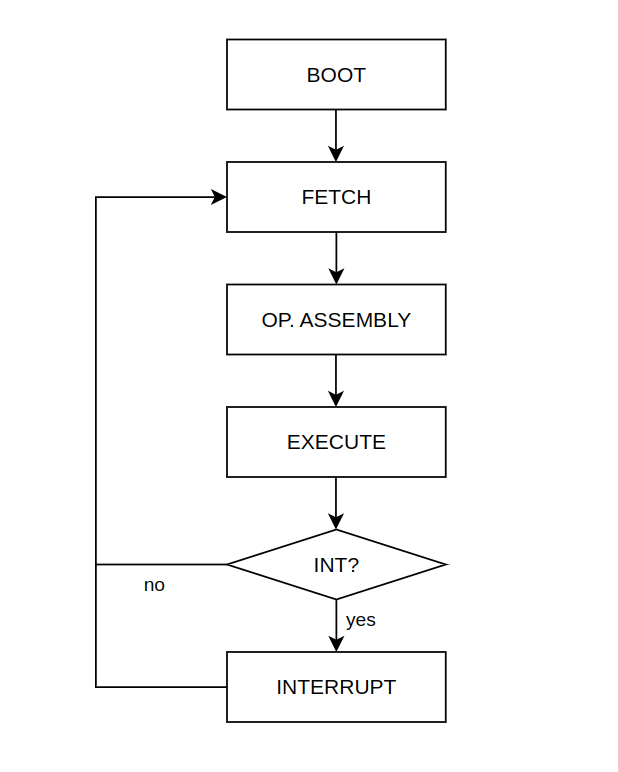
\includegraphics[width=0.5\textwidth]{img/BootInt.png}
    \caption{Ciclo di esecuizone con interrupt}\label{img:bootint}
\end{figure}
Quindi quando le interruzioni sono scatenate vanno ad effettuare una chiamata a subroutine particolare, tale chiamata è detta ISR (Interrupt-Services-Routine). Tale situazione, quindi, ferma il sistema dalla sua normale esecuzione del programma per dare priorità alla gestione dell'interruzione. Questo, quindi, apre molti dubbi su come gestire lo stato in cui si trova la macchina, poichè se quando torno dalla ISR, ho cambiato qualche registro significativo si potrebbe compromettere il normale funzionamento del programma. In generale i due registri che richiedono l'obbligo di essere salvari sono i registri: \textbf{SR(Status register)} e il \textbf{PC(Program Counter)}. In generale, i registri che vado a salvare in questo passaggio sono anche detti: \textbf{Descrittore di processo}, tali registri, quindi, descrivono lo stato di funzionamento del mio processore quando poi è stato prelazionato dalla mia ISR. Ciò mi permette di proseguire ancora con la normale esecuzione del programma prefissato.

\subsubsection{Gestione delle Interruzioni}
Una volta definito cosa sono le interruzioni è di fondamentale importanza capire come il processore le gestisce. Le principali modalità di gestione delle interruzioni sono due e sono:
\begin{itemize}
    \item \textbf{Vettorizzate}: Ogni livello di priorità di interrupt è collegato al processore. I fili di collegamento per le interrupt sono limitati, quindi più dispositivi possono collegarsi sullo stesso cavo di interrupt. Il processore, quindi, per identificare il dispositivo che ha scatenato l'Interrupt va a controllare i bus, su cui il dispositivo ha caricato il suo codice identificativo. Identificare il dispositivo, vuol dire identificare la tipologia di ISR da andare ad utilizzare. Gli indirizzi degli entry-point delle varie periferiche sono memorizzati in memoria a partire dall'indirizzo 0 a seguire per 256 locazioni di 4 byte. Tali locazioni si dividono nel seguente modo:
    \begin{itemize}
        \item \textbf{Funzioni speciali}: Da 0 a 24, gli entry-point identificano delle funzioni speciali o di gestione aritmentica
        \item \textbf{Interruzioni autovettorizzate}: da 25 a 31 sono indicizzate le locazioni per il funzionamento autovettorizzato
        \item \textbf{Trap}: da 32 a 47 sono indicizzate le funzioni per la gestione dei Trap
        \item \textbf{Utilizzabili}: da 48 a 256 sono locazioni disponibili per l'inserimento degli entry-point per la gestione di diverse periferiche
    \end{itemize}
    \item \textbf{Autovattorizzate}: A differenza del caso vettorizzato, evita la lettura del codice identificativo, poichè ogni livello di interrupt è collegato al vettore delle ISR autovettorizzate e permette di selezionare in maniera "ignorante" l'ISR alla locazione della tipologia di priorità inserita
\end{itemize}

\subsubsection{PIC} \label{par:PIC}
In generale, nel caso di sistema \textbf{vettorizzato}, viene in aiuto il componente \textbf{PIC (Programmable Interrupt Controller)} [\ref{img:PIC}].
Il PIC è un dispositivo che permette di arricchire le
modalità di gestione delle interruzioni. Grazie alla programmazione di questo oggetto, possiamo assegnare alle varie periferiche non una sola linea di interruzione con una specifica ISR, ma possiamo esplorare tutto il vettore delle interruzioni, che in teoria è costituito da 256 locazioni. In sostanza, il PIC permette di usare interrupt vettorizzate, ovvero il dispositivo fornisce sul data bus un vettore di 8 bit che rappresenta l’indice all’interno della tabella delle interruzioni corrispondente all’indirizzo della corretta ISR. Nel M68k questo protocollo è simulato con il PIC: Il dispositivo non scrive sul data bus il vettore di 8 bit, ma comunica l’interruzione al PIC che si occuperà di capire qual è il vettore corrispondente al dispositivo interrotto. Il PIC estende la gestione delle interruzioni del processore M68K introducendo nuove funzionalità, come la gestione prioritaria, la mascheratura delle interruzioni e le linee di interrupt. Il dispositivo ha in uscita verso il processore una linea di interruzione INT e una linea di INTA (acknowledgement) , mentre ha in ingresso 8 linee di interruzioni differenti, a priorità decrescente (0 massima, 7 minima). Più dispositivi possono essere connessi in cascata, fino a 8 per un massimo di 64 linee di interruzione.
Il PIC accetta richieste di interruzione dai dispositivi di IO connessi alle sue linee e determina, a seconda dell’algoritmo di gestione prioritaria selezionato, quale delle interruzioni simultaneamente attiva ha la priorità più alta. Dopodiché trasmette un segnale sulla linea INT al processore, attende un segnale su INTA (handshaking) e poi trasmette sul bus dati il vettore di 8 bit a cui corrisponde la corretta interruzione sulla tabella delle interruzioni.
Il Control Register interno al PIC permette di configurare la gestione prioritaria mediante un’opportuna modifica:
\begin{itemize}
    \item \textbf{Fully nested}: le richieste di interruzione sono ordinate secondo uno schema a priorità fissa che va da IR0 a IR7;
    \item \textbf{Round Robin}: Schema prioritario a rotazione, ovvero la linea di interruzione più prioritaria appena servita diventa la meno prioritaria dopo il servizio;
    \item \textbf{Maschera interruzioni} consente l’inibizione o l’abilitazione delle linee di interruzione.
\end{itemize}

Il modo di operazione scelto dev essere configurato in fase di inizializzazione del PIC, ma può anche essere dinamicamente cambianto da un apposito programma di gestione.
L’Interrupt Request Register (IRR) riceve in ingresso le 8 linee di interruzione provenienti dalle periferiche collegate e ne memorizza lo stato. L’input a questo registro è gestito da un circuito integrato che si occupa della gestione prioritaria delle interruzioni, mentre l’output è il registro In Service Register (ISR) in cui vengono memorizzati solo i segnali di interruzione da servire in accordo alla maschera (IMR). Il Type Register (TR) è un registro di 8 bit che memorizza nei 5 bit più significativi il valore base del vettore da scrivere in output sul bus dati, mentre nei 3 meno significativi uno spiazzamento in accordo alla linea interrompente. Dopo il servizio, l’i-esimo bit di IRR è automaticamente cancellato per riuovere la causa di interruzione.

\begin{figure}
    \centering
    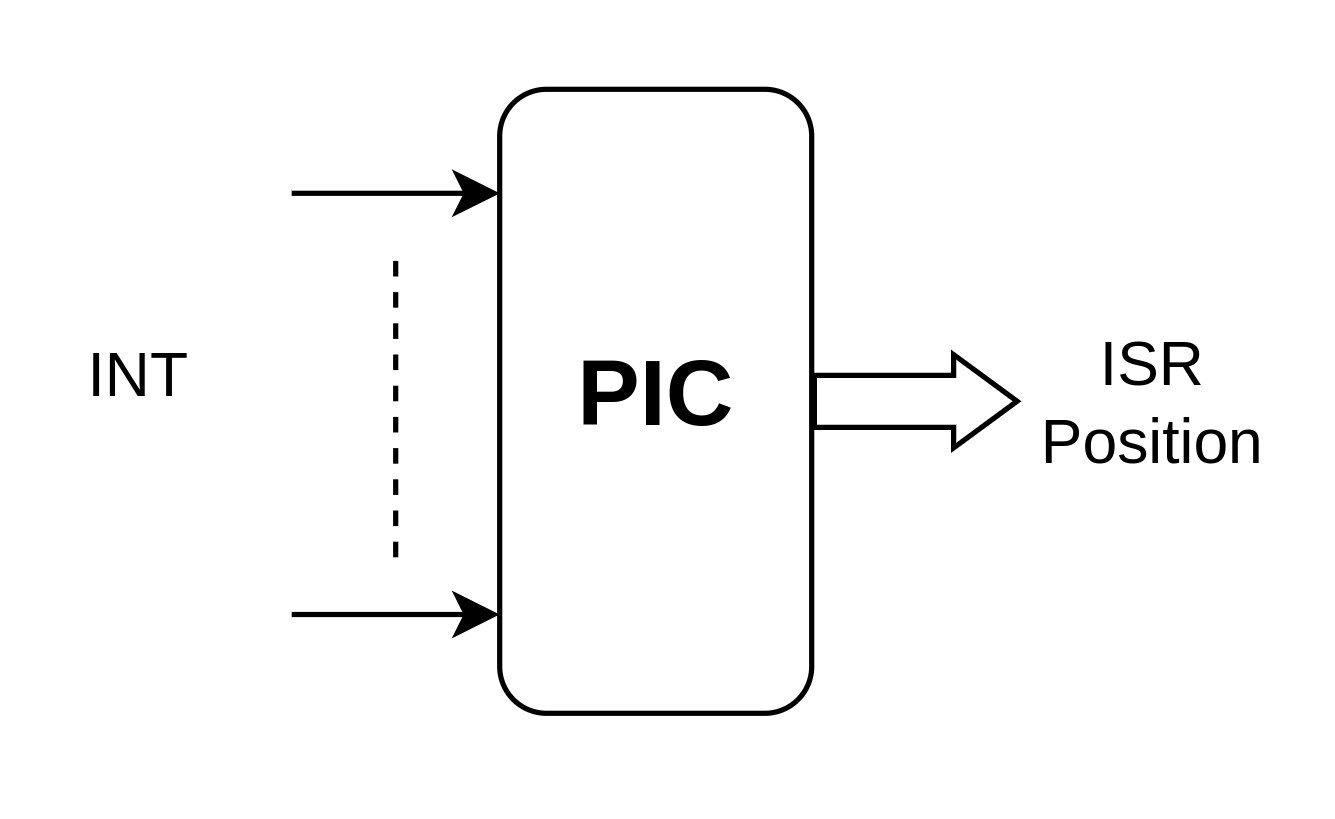
\includegraphics[width=0.7\textwidth]{img/PIC.png}
    \caption{PIC(Programmable Interrupt Controller)}\label{img:PIC}
\end{figure}

\begin{figure}
    \centering
    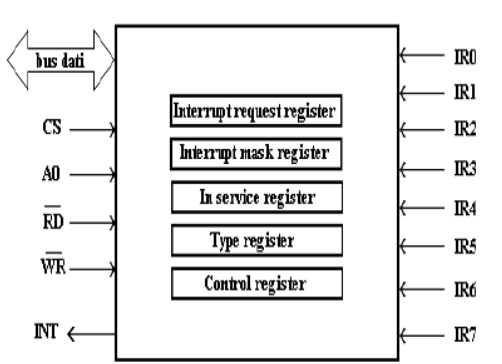
\includegraphics[width=0.5\textwidth]{img/PIC2.png}
    \caption{PIC: modello di programmazione}\label{img:PIC2}
\end{figure}


\subsection{Estensione del modello IO generale}
Un modello di architettura dotato solo di PIA (\ref{par:PIA}) è limitato: può gestire solo caratteri, ha a disposizione solo 7 interruzioni e può generare attese infinite con il protocollo di handshaking.
Per risolvere questi problemi, vengono introdotti nuovi elementi nell'architettura: \textbf{DMA} per gestire il trasferimento di messaggi invece di caratteri, \textbf{PIC} (\ref{par:PIC}) per superare la limitazione sul numero di ISR indirizzabili e \textbf{TIMER} per gestire la temporizzazione e il risolvere il problema delle attese infinite (\ref{img:IO_ESTESO}).

\begin{figure}[!ht]
    \centering
    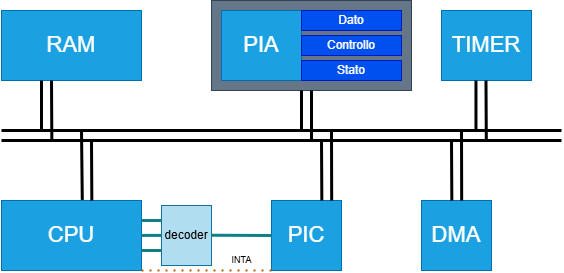
\includegraphics[width=0.75\textwidth]{img/Schema_IO_1.png}
    \caption{Modello IO esteso - schema logico}
    \label{img:IO_ESTESO}
\end{figure}

Il timer espone il modello di programmazione Registro di stato, Registro di valore e Registro di Modo. Nel registro di valore di solito è scritto un istante in cui il timer si "sveglia" e genera un'interruzione: infatti il timer possiede una linea con la quale può comunicare un'interruzione.

 % Capitolo 2
% Aggiungi altri file di capitoli se necessario

\chapter{Esercitazioni}
In questo capitolo saranno affrontate tutte le tematiche riguardanti le esercitazioni di maggiore interesse. Quindi saranno approfondite le sole esercitazioni in cui sono stati affrontati anche degli argomenti teorici importanti.

\section{Debunk esercizi PIA}
In questo paragrafo verrà commentato il codice diffuso sul canale Teams e presentato a lezione relativo alle esercitazioni sulla PIA (Marzo 2025).

% \subsection{Esercizio 2}\label{par:es_1_2}
% Il programma serve a provare una semplice configurazione costituita da due sistemi S1 ed S2 dotati entrambi di un processore M68000, una ROM di 8K (addr \$0-\$1FFF), una RAM di 10K (addr \$8000-\$A7FF) e un device parallelo PIA mappato a \$2004. I due PIA sono interconnessi tra loro e mediante un protocollo di handshaking consentono ai due sistemi di scambiarsi un messaggio. In particolare, il sistema S1 trasferisce un vettore di N caratteri verso il sistema S2 sul porto parallelo. Il messaggio si trova in un'area di memoria del sistema S1 e viene salvato in una ulteriore area di memoria nel sistema S2. Questa volta, anche la trasmissione è gestite tramite interrupt e non tramite polling come nel paragrafo \ref{par:es_1_1}.

% \subsubsection{Sistema S1}
% Questo driver serve per la programmazione del sistema S1, che effettua il trasferimento sotto interrupt.
% Per quanto riguarda l'area dati valgono le stesse considerazioni fatte per l'esercizio 1 (\ref{par:es_1_1_1}), con l'aggiunta dell'allocazione di una variabile COUNT anche per il trasmettitore. 

% \begin{lstlisting}
%     ***AREA MAIN***
% 	ORG    $8200

% PIADB	EQU    $2006	;indirizzo di PIA-B dato, usato in output 
% PIACB	EQU    $2007	;indirizzo di PIA-B controllo

% MAIN	JSR    DVBOUT	;inizializza PIA porto B in output

% 	MOVEA.L	#PIACB,A1	;indirizzo registro di controllo CRB
% 	MOVEA.L	#PIADB,A2	;indirizzo registro PRB
% 	MOVEA.L	#MSG,A0	;indirizzo area messaggio

% 	MOVE.W	SR,D0	;legge il registro di stato
% 	ANDI.W	#$D8FF,D0 ;maschera per reg stato (stato utente, int abilitati)
% 	MOVE.W	D0,SR	;pone liv int a 000

% * invio primo carattere:	
% INVIO1	MOVE.B	(A2),D1;lettura fittizia da PRB => serve per azzerare CRB7 poiche in generale non sappiamo se la macchina e' in reset
% 	    MOVE.B	(A0),(A2)	;dato su bus di PIA porto B: dopo la scrittura di PRB, CB2 si abbassa
% 					;cio fa abbassare CA1 sulla porta gemella dell'altro sistema generando 
% 					;un'interruzione che coincide con il segnale DATA READY

% 	    MOVE.B	#1,COUNT
% LOOP  	JMP LOOP	;ciclo caldo dove il processore attende interrupt		
% \end{lstlisting}

% Vediamo nel dettaglio la subroutine CVBOUT, ovvero il sottoprogramma reponsabile della configurazione del porto B come porto di output e del protocoloo handshaking.

% \begin{lstlisting}
%     DVBOUT	MOVE.B	#0,PIACB		;seleziona il registro direzione di PIA porto B 
% 	MOVE.B	#$FF,PIADB	  		;accede a DRB e pone DRA=1 : le linee di B sono linee di output	
% 	MOVE.B	#%00100101,PIACB   	;imposta il registro di controllo 
% *								;i bit CRB7 e CRB6 sono a sola lettura	
% 	RTS
% \end{lstlisting}

% Valgono le stesse considerazioni fatte nel caso dell'esercizio (\ref{par:es_1_1_1}). Questa volta, il byte da scrivere nel registro di controllo è 00100101: b1b0 = 01 significa che le interruzioni vengono propagate al processore tramite il flag CRB7 e che si alza sul fronte di discesa di CA1. Il flag di interruzione CRB7 torna basso in seguito ad un'operazione di lettura su PRB (\textbf{per questo è necessaria la lettura fittizia}); b2=1 signfica che il prossimo accesso ad indirizzo pari sarà sul registro dati PRB; b5b4b3=100 significa protocollo di handshaking e valgono le stesse considerazioni fatte per l'esercizio (\ref{par:es_1_1_1}). 

% Procedendo con il main, è necessario inviare dal codice il primo carattere, perchè i successivi verrano gestiti dalla ISR relativa. 
% Vediamola quindi nel dettaglio: La pia-A dell'altro sistema ha appena letto un carattere e scatena l'handshake che genera una interrupt
% su questo sistema: la ISR invia il prossimo carattere prelevandolo dalla memoria se ce ne sono ancora da trsmettere.
% ISR a \$8800 associata all' interrupt di liv. 4  \#vect 28  mappato a \$70 della ROM.

% \begin{lstlisting}
%     ORG $8800		

%     INT4    	MOVE.L	A1,-(A7)		;salvataggio registri
%         MOVE.L	A0,-(A7)
%         MOVE.L	D0,-(A7)
%         MOVE.L	D1,-(A7)
%         MOVE.L	D2,-(A7)
    
%         MOVEA.L	#PIADB,A1
%         MOVEA.L	#MSG,A0	;indirizzo area di salvataggio
%         MOVE.B	DIM,D0	;dim del messaggio
%         MOVE.B	COUNT,D1	;contatore corrente degli elementi ricevuti
    
%         CMP.B	D1,D0
%         BEQ	FINE
        
%     INVIO	MOVE.B	(A1),D2            ;lettura fittizia da PRB => serve per azzerare CRB7 dopo il primo carattere, altrimenti resta settato con l ack
%         MOVE.B	(A0,D1),(A1)	;carattere corrente da trasferire in D2;
%     *					;dato su bus di PIA porto B: dopo la scrittura di PRB, CB2 si abbassa
                    
%         ADD.B	#1,D1			;aggiorno il contatore degli elementi trasmessi
%         MOVE.B	D1,COUNT
    
%     FINE	MOVE.L  (A7)+,D2		;ripristino registri 
%         MOVE.L  (A7)+,D1
%         MOVE.L  (A7)+,D0	
%         MOVE.L  (A7)+,A0
%         MOVE.L  (A7)+,A1
        
%         RTE
% \end{lstlisting}

\subsection{Esercizio 1}
Il programma serve a provare la configurazione \textbf{communic asincrona} costituita da due sistemi simmetrici ciascuno con un processore M68000, una ROM di 8K (addr \$0-\$1FFF), una RAM di 10K (addr \$8000-\$A7FF), un device parallelo PIA mappato a \$2004, un device seriale di tipo TERMINAL mappato a \$2000.
I due PIA sono interconnessi e mediante un protocollo di handshaking consentono ai due sistemi di scambiarsi i caratteri digitati sul dispositivo TERMINAL. I device interagiscono con i rispettivi processori mediante le linee di interruzione utilizzando un meccanismo di  
interrupt autovettorizzato (TERMINAL e PIA non supportano le int.vettorizzate). 
In particolare i dati immessi da tastiera sono acquisiti, alla pressione del tasto ENTER, mediante interruzione di livello 1, che corrisponde al vettore 25 mappato in area ROM alla locazione \$64: in tale locazione è contenuto l'indirizzo della ISR in RAM (\$8500).
Nella ISR, il dato viene inviato alla sezione A del dispositivo parallelo PIA per la trasmissione verso il dispositivo 
PIA connesso all'altro sistema.
La ricezione di un carattere sul dispositivo PIA e' gestita mediante interruzione di livello 3, che corrisponde al vettore 27 mappato in area ROM alla locazione \$6C: in tale locazione è contenuto l'indirizzo della ISR in RAM (\$8700). All'arrivo dell'interrupt la ISR acquisisce il dato e lo invia al terminal per la visualizzazione.
Un'ulteriore ISR mappata sull'autovettore 26 gestisce le condizioni di buffer full sul TERMINAL.
Tale ISR invia sulla PIA i 256 caratteri nel buffer.
Nell'esercizio vedremo uno stesso programma caricato per entrambi i sistemi speculari, sfruttando il meccanismo delle interruzioni: infatti le interruzioni generate dai dispositivi (autovettorizzate) saranno diverse e permetteranno comportamenti diversi tra i due sistemi.


\begin{lstlisting}
    BEGIN	ORG    $8200


    PIADA	EQU    $2004	;indirizzo di PIA-A dato, usato in input
    PIACA	EQU    $2005	;indirizzo di PIA-A stato/controllo
    PIADB	EQU    $2006	;indirizzo di PIA-B dato, usato in output 
    PIACB	EQU    $2007	;indirizzo di PIA-B controllo
    
    TERD	EQU    $2000    ;indirizzo di TERMINAL registro dato
    TERC	EQU    $2001	;indirizzo di TERMINAL registro stato/controllo
    
            JSR    DVAIN	;inizializza PIA porto A
            JSR    DVBOUT	;inizializza PIA porto B
            JSR    DVTER	;inizializza terminal
            MOVE.W	SR,D0	;legge il registro di stato
            ANDI.W	#$D8FF,D0 ;maschera per reg stato (stato utente, int abilitati)
            MOVE.W	D0,SR	;pone liv int a 000
    
    LOOP  	JMP LOOP	;ciclo caldo dove il processore attende interrupt	
\end{lstlisting}

Notiamo subito che in questo esercizio è necessario configurare il dispositivo PIA sia sul porto A che sul porto B per entrambi i sistemi, perchè vogliamo garantire una comunicazione \textit{FULL DUPLEX} come mostrato in figura \ref{img:PIA_FD}. Come negli altri esercizi, configuriamo il porto B per la scrittura e il porto A per la lettura. 

\begin{figure}[!ht]
    \centering
    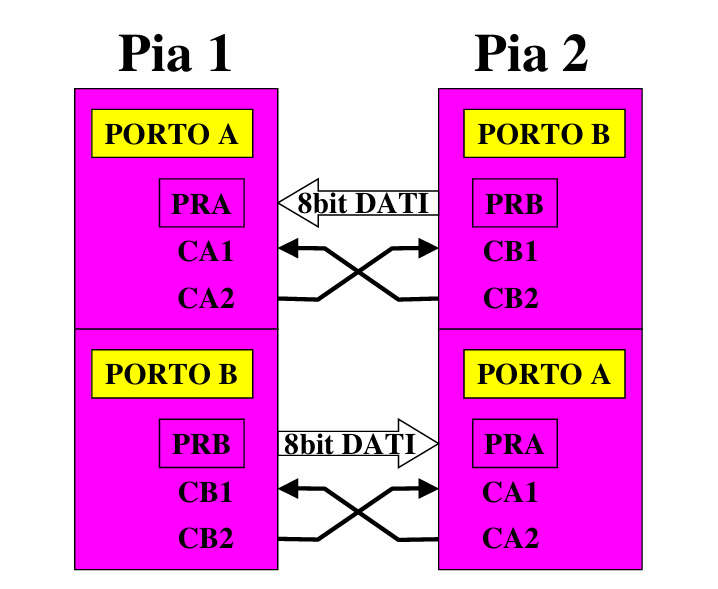
\includegraphics[width=0.75\textwidth]{img/PIA_fd.png}
    \caption{Configurazione Full Duplex}\label{img:PIA_FD}
\end{figure}

Le routine dedicate alla configurazione dei porti A e B sono uguali a quelle viste nell'esercizio 2 di questa sezione (\ref{par:es_1_2}).
La routine dedicata alla configurazione del terminale consta di una sola istruzione e ritorna:

\begin{lstlisting}
    DVTER	MOVE.B	#$3f,TERC	;seleziona indirizzo stato/controllo
	RTS		
\end{lstlisting}

In pratica viene soltanto scritto il bye 00111111 nel registro di controllo/stato del terminale, il cui significato è chiarito dall'immagine \ref{img:terminal_cfg}.

\begin{figure}[!ht]
    \centering
    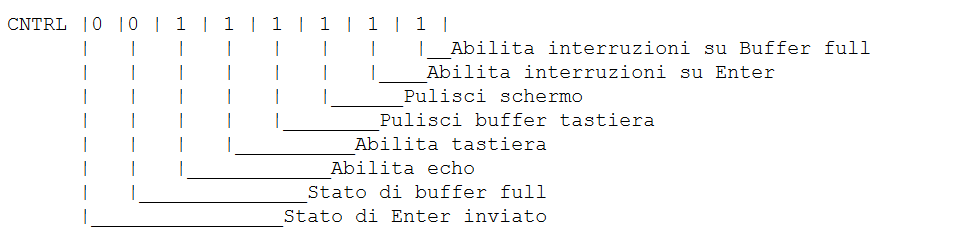
\includegraphics[width=0.5\textwidth]{img/terminal_ctrl.png}
    \caption{Configurazione registro controllo/stato del terminale}
    \label{img:terminal_cfg}
\end{figure}

Dopodichè, il main entra in un ciclo idle in cui attende le interruzioni (dopo averle abilitate sul registro di stato).
Vediamo nel dettaglio la ISR per la gestione dato proveniente dalla tastiera di TERMINAL e spedito, per tramite del PIA porto B, all'altro sistema.
ISR associata all'interrupt di liv. 1, \#vect 25 mappato a \$64 della ROM con ISR a \$8500. 

\begin{lstlisting}
    ORG	$8500		ricevi da tastiera
    INT1	MOVE.L	A0,-(A7)		;push di A0,A1,A2,D0,D1 in stack supervisor
        MOVE.L	A1,-(A7)
        MOVE.L	A2,-(A7)
        MOVE.L	D0,-(A7)
        MOVE.L	D1,-(A7)
        MOVEA.L	#TERD,A0
        MOVEA.L	#PIADB,A1
        MOVEA.L	#PIACB,A2
    
    INPUT	MOVE.B	(A0),D0			;acquisisci dato da terminal
    
    *trasferisci il carattere letto alla PIA-B con handshaking
            MOVE.B  (A1),D1         ;lettura fittizia 
            MOVE.B  D0,(A1)         ;Dato su bus di PIA porto B: dopo la scrittura di PRB, CB2 si abbassa
    *								;cio fa abbassare CA1 sulla porta gemella dell'altro sistema generando 
    *								;un'interruzione che coincide con il segnale DATA READY
        
    ciclo2	MOVE.B	(A2),D1			;In attesa di DATA ACKNOWLEDGE
        ANDI.B	#$80,D1				;aspetta che CRB7 divenga 1
        BEQ	ciclo2
                
    *fine trasferimento e handshaking
        
        CMP.B   	#13,D0		;Se il carattere ricevuto  ENTER	
        BNE     	INPUT		;termina altrimenti prossimo carattere
        ORI.B	#$1C,TERC		;riabilita tastiera ,pulisce buffer e video
        MOVE.L 	(A7)+,D1		;ripristino di D0,D1,A2,A1,A0
        MOVE.L	(A7)+,D0
        MOVE.L	(A7)+,A2
        MOVE.L	(A7)+,A1
        MOVE.L	(A7)+,A0
        RTE
\end{lstlisting}

In questo caso è presente per forza di cose un ciclo improduttivo (ciclo2) perchè bisogna procedere sequenzialmente al set di istruzioni successivo che prevede un salto a INPUT se il carattere ricevuto non è quello finale (ENTER). Dopodichè resetta il terminale riabilitando tastiera e pulendo buffer e video scrivendo nel registro di controllo in accordo a quanto esposto nella figura \ref{img:terminal_cfg}, e ritorna.

Procediamo vedendo la ISR per il \textit{buffer full}: praticamente è identica a quella per l'acquisizione del messaggio in seguito a ENTER, ma in questo caso vengono inviati tutti e 256 i caratteri conservati nel buffer del terminale.
ISR a \$8600 associata all'interrupt di livello 2 \#vect (24+2) => mappato a 4*26 = 104 = \$68.

\begin{lstlisting}
    ORG	$8600		
    INT2	MOVE.L	A0,-(A7)		;push di A0,A1,A2,D0,D1 in stack supervisore
        MOVE.L	A1,-(A7)
        MOVE.L	A2,-(A7)
        MOVE.L	D0,-(A7)
        MOVE.L	D1,-(A7)
        MOVE.L	D2,-(A7)
        MOVEA.L	#TERD,A0
        MOVEA.L	#PIADB,A1
        MOVEA.L	#PIACB,A2
        MOVE.B	#255,D2		;#caratteri da trasferire
        
    SWAP	MOVE.B	(A0),D0			;acquisisci dato da terminal
    
    *trasferisci il carattere letto alla PIA-B con handshaking
        MOVE.B  (A1),D1         ;lettura fittizia => serve per azzerare CRB7 dopo il primo carattere, altrimenti resta settato con l ack
        MOVE.B  D0,(A1)         ;Dato su bus di PIA porto B: dopo la scrittura di PRB, CB2 si abbassa
    *							;cio fa abbassare CA1 sulla porta gemella dell'altro sistema generando 
    *							;un'interruzione che coincide con il segnale DATA READY
        
        
    ciclo3	MOVE.B	(A2),D1		;In attesa di DATA ACKNOWLEDGE
        ANDI.B	#$80,D1		;aspetta che CRB7 divenga 1
        BEQ	ciclo3
                
    *fine trasferimento e handshaking
            
        DBRA    	D2,SWAP	;contatore di bit inviati	
        ORI.B	#$1C,TERC	;riabilita tastiera ,pulisce buffer e video
        MOVE.L	(A7)+,D2	;ripristino di D0,D1,A2,A1,A0
        MOVE.L 	(A7)+,D1
        MOVE.L	(A7)+,D0
        MOVE.L	(A7)+,A2
        MOVE.L  	(A7)+,A1
        MOVE.L  	(A7)+,A0
        RTE
\end{lstlisting}

L'ultima interruzione è quella che scatena il porto A in seguito alla ricezione di un carattere. 

\begin{lstlisting}
    ORG $8700		

    INT3    	ANDI.B		#%11101001,TERC	;disabilita: tastiera,cancella video,interruzioni su enter		 
        MOVE.L  A1,-(A7)		;salvataggio registri
        MOVE.L  A0,-(A7)
        MOVE.L  D0,-(A7)
    
        MOVEA.L  #TERD,A0	;inizializzazione indirizzi device
        MOVEA.L  #PIADA,A1
        
        MOVE.B 	(A1),(A0)	;acquisisce il carattere e lo trasferisce a Terminal
    *						;la lettura da PRA fa abbassare CRA7 e CA2 => nell'altro sistema si abbassa CB1
    *						;cio corrisponde all'attivazione di CRB7 che funge da DATA ACKNOWLEDGE
        
        MOVE.L  (A7)+,D0		;ripristino registri 
        MOVE.L  (A7)+,A0
        MOVE.L  (A7)+,A1
        
        ORI.B	#$12,TERC	;riabilita tastiera e interruzioni su enter 
        RTE
    
    
        END	BEGIN
\end{lstlisting}

\subsection{Considerazioni finali}
In conclusione, è utile chiarire che le linee di interruzione IRQA e IRQB sono direttamente collegate ai flag CRA7 e CRB7, che si alzano quando c'è una transizione attiva dei segnali CA1/CB1 rispettivamente.
I flag di interruzione CRA7/CRB7 vengono automaticamente abbassati dopo un'operazione di READ
sul porto corrispondente, e questo è il motivo per cui nella parte software è necessaria la \textit{lettura fittizia}. 
Per quanto riguarda i bit del registro di stato/controllo del dispositivo PIA, in questa esercitazione abbiamo visto la configurazione per il protocollo di comunicazione handshaking. Le altre modalità, definite in base ai bit 5,4 e 3 dei registri di controllo,disciplinano il momento in cui CA2/CB2 deve essere rialzato, quindi non cambia nulla
dal punto di vista delle funzionalità.
\section{TAS (Test and Set)}

\textbf{TAS} è un'istruzione che:
\begin{itemize}
    \item \textbf{Controlla} se il bit più significativo dell'operando è 0 (semaforo libero);
    \item \textbf{Set} del bit più significativo a 1 (semaforo occupato) nel caso lo trovi libero. 
\end{itemize}

A seguito dell'operazione i bit N e Z dello SR vengono aggiornati. Questa operazione è atomica (indivisibile), quindi usa un solo ciclo read-modify-write. La sua principale applicazione è nei sistemi multiprocessore: infatti un processore che esegue TAS non può essere interrotto tra la fase di Test e la fase di Set, rendendo consistente l'operazione di acquisizione del semaforo. 
Il metodo di indirizzamento è indiretto o tramite registro. 

\subsection{Esercizio 1} \label{par:esercizio_2_1}
Due nodi B e C inviano K messaggi da N caratteri al nodo A, ognuno tramite una periferica PIA. Senza particolari ipotesi semplificative sulla priorità di un nodo rispetto ad un altro, scrivere il codice assembler eseguito dal nodo A in modo che:

\begin{itemize}
    \item Se il nodo B trasmette un messaggio ad A, A deve terminare la ricezione dell'intero messaggio prima di ricevere un eventuale messaggio da C.
    \item Analogamente, se il nodo C trasmette un messaggio ad A, A deve terminare la ricezione dell'intero messaggio prima di ricevere un eventuale messaggio da B. 
\end{itemize}

Il collegamento tra i dispositivi avviene tramite PIA secondo il meccanismo indicato precedentemente. Per la configurazione fare riferimento alla figura \ref{img:TAS_1}

\begin{figure} [!ht]
    \centering
    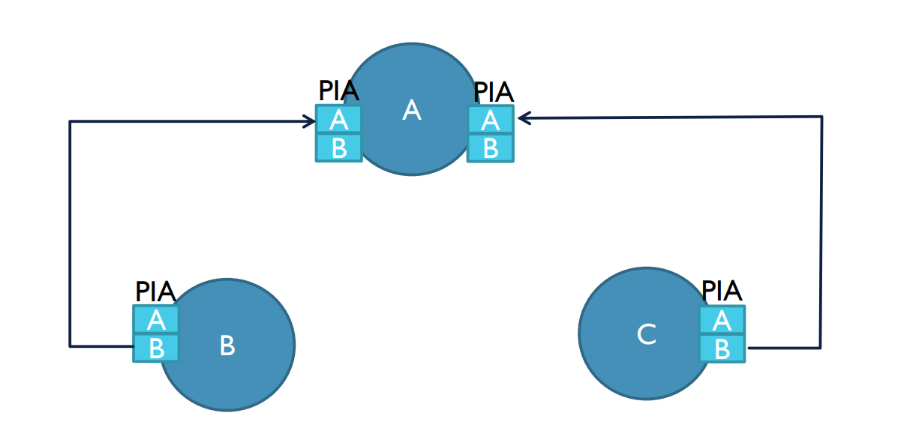
\includegraphics[width=0.5\textwidth]{img/TAS_1.png}
    \caption{Schema logico}\label{img:TAS_1}
\end{figure}

Possiamo considerare il nodo A come una risorsa condivisa dai nodi B e C. Siamo nel caso in cui è possibile utilizzare l'istruzione TAS: Prima di effettuare l'invio del messaggio, B e C devono verificare che A non sia impegnato con l'altro nodo. Questo è possibile farlo se A definisce una variabile \textit{possesso}, dove il valore 0 indica il possesso di B, 1 indica il possesso di C, -1 indica risorsa libera. L'accesso alla variabile \textit{possesso} deve essere mutualmente esclusivo, per evitare race conditions. Per questo motivo la variabile è acceduta tramit un lock, controllato e settato tramite TAS. 
Poichè stiamo utilizzando la PIA in configurazione tale per cui la ricezione di un messaggio dal nodo A causa interruzione, possiamo programmare l'ISR di A relativa alla ricezione di un messaggio da parte di B o da parte di C. 

\begin{itemize}
    \item \textbf{ISRB}: Per prima cosa si controlla che A non sia impegnato nella comunicazione con C, controllando la variabile possesso (in mutua esclusione). Se il possesso è di B (0) o è libero (-1) allora si può procedere all'invio, altrimenti B aspetta. 
    \item \textbf{ISRC}: Per prima cosa si controlla che A non sia impegnato nella comunicazione con B, controllando la variabile possesso (in mutua esclusione). Se il possesso è di C (1) o è libero (-1) allora si può procedere all'invio, altrimenti C aspetta.
\end{itemize}

Questo meccanismo è pericoloso in quanto permette il DeadLock. Serve un meccanismo per riprendere la ricezione sospesa. Il motivo per cui una ricezione possa essere sospesa è un'interruzione di priorità maggiore o un malfunzionamento della periferica. 

vediamo lo pseudocodice relativo alla ISRB:

\begin{lstlisting}[language=C]
    if (sem == verde){      \\istruzione atomica TAS
        sem = rosso;
        if (possesso != 1){ \\possesso non di C
            possesso = 0;
            sem = verde;
            leggo_car_b();
            car_counter_b++;
            if (car_counter_b==N){ \\fine trasmissione
                if(c_sospeso){
                    possesso = 1; \\possesso di C
                    leggo_car_c();
                    car_counter_c++;
                }
                else{
                    possesso=-1;
                }
            }
        }
        else{
            sem = verde;
            leggo_car_c();
            car_counter_c++;
        }
        return 0;
    }
    return 0;
\end{lstlisting}

Nel codice vediamo che tramite l'istruzione TAS controlliamo se il semaforo è verde e lo settiamo subito a rosso. Quindi, se il possesso non è di C, B prende il possesso e reimposta il semaforo a verde, dopodichè procede con la lettura del prossimo carattere. Se il messaggio è finito, se C è sospeso C viene sbloccato attraverso la lettura del carattere di C, altrimenti viene liberato il possesso. Se il possesso è già di C, C potrebbe aver provato ad accedere alla sezione critica (invio del messaggio) mentre B controllava in mutua esclusione il possesso. In questo caso, C viene sbloccato attraverso la lettura di un carattere. Se in primo luogo B trova il semaforo rosso, B viene sospeso.
Per verificare se B o C sono sospesi, si controlla nel registro di stato se CRA7B o CRA7C sono alti (interruzione pendente). 
Lo pseudocodice della ISRC è praticamente speculare a quello presentato sopra. 


\subsection{Esercizio 2 - Prova intercorso 2023}
Un sistema è compoto da 3 unità (A,B,C) tra loro collegate mediante due periferiche parallele che interconnettono A con B e A con C rispettivamente. Il sistema opera effettuando k iterazioni (k>2), in ciascuna delle quali A deve ricevere globalmente 2 messaggi di N caratteri da B e 1 messaggio di N caratteri da C (N>2). I messaggi da B e da C possono essere ricebuti in un ordine qualsiasi ma non deve essere mai possibile ricevere caratteri appartenenti a messaggi diversi intervallati tra di loro.
Vediamo lo pseudocodice relativo alla ISRB:

\begin{lstlisting}[language=C]
    if (sem == verde){      \\istruzione atomica TAS
        sem = rosso;
        if (possesso != 1 && end_B == 0){ 
            possesso = 0;
            sem = verde;
            leggo_car_b();
            car_counter_b++;
            if(car_counter_b == N){
                mex_counter_b++;
                if(mex_counter_b == N_mex_b){
                    end_B = 1;
                }
                if(c_sospeso){
                    possesso = 1; \\possesso di C
                    leggo_car_c();
                    car_counter_c++;
                }
                else{
                    possesso=-1;
                }
            }
        }
        else{
            sem = verde;
            leggo_car_c();
            car_counter_c++;
        }
        return 0;
    }
    return 0;
\end{lstlisting}

La differenza rispetto all'esercizio \ref{par:esercizio_2_1}, B in questo caso per procedere deve controllare sia che la variabile possesso non sia di B, sia che A non abbia già ricevuto il numero di messaggi per quell'iterazione. Dopo la ricezione del carattere, non solo viene gestito il contatore relativo ai caratteri nel messaggio, ma anche un contatore che tiene conto del numero di messaggi ricevuti nella corrente iterazione. Se questo numero diventa uguale a N, si pone $end_B = 1$, e alla successiva interruzione non si riceverà alcun carattere, ma si sveglierà C se necessario e si uscirà. 


\appendix

\chapter{Appendice}

+\section{Asim e Asimtool}
Per la scrittura e la simulazione dei codici, saranno utilizzati i seguenti strumenti:
\begin{itemize}
    \item \textbf{ASIM}: Strumento per la simulazione del motorola 68k
    \item \textbf{ASIM-Tool}: Editor di testo e compilatore dei file .a68
\end{itemize}

\subsection{Asimtool}

Per asimtool, dopo aver scritto il file bisogna generare il file \.LIS, che poi sarà inserito all'interno del simultaore ASIM\. Tale file va generato secondo il seguente path: 
\\
\textbf{Assemble -> Assemble File <Nome\_File>.a68}
\\
Fatta tale operazione, nella cartella dove vi è salvato il file \.a68 dovrebbe essersi generato il file \.LIS
\\
Nel caso ci fossero particolari errori, asimtool li mostrerà a video specificando le righe su cui tali errori si presentano. Si invita a tenere ben cura della spaziatura tra i vari comandi e la loro leggittima posizione


\subsection{ASIM}
Una volta generato il file \.LIS con ASIM-tool, aprire ASIM ed impostare l'ambiente. Per impostare l'ambiente è richiesto un file cfg, che riporta i vari componenti che saranno mostrati all'interno del simulatore (tipo la memoria, il processore ecc.).
Il file base.cfg può essere trovato sui canali ufficiali degli studenti o può essere richiesto al professore. Tale file non contiene altro che una lista di componenti che verranno poi mostrati all'interno del simulatore.
Una volta aperto il file bisogna seguire il seguente path:
\\
\textbf{Window -> Tile}
\\
Tale opzione ci permette di poter vedere tutte le schermate aperte in maniera ordinata. Successivamente all'ordinamento delle schermate, bisogna "attivare" la configurazione, per fare ciò bisogna premere su di un tasto nella barra degli strumenti in Alto con illustrata una grossa I.
Una volta attivato il nostro ambiente, tenere cura di selezionare la finestra su cui c'è scritto di caricare il \.LIS. Una volta fatto questo in alto, tra i menu comparirà una nuova voce, ovvero: \textbf{Proc\_Unit}.
Una volta apparso tale menu basterà seguire il seguente path per poter selezionare il file \.LIS:
\\
\textbf{Proc\_Unit -> Load Assembler}
\\
Tale comando permetterà di poter caricare il file \.LIS generato da Asimtool, che dovrà essere selezionato appositamente tramite il file explorer.
Una volra caricato il file \.LIS bisognerà solo eseguire il programma.
Si consiglia, prima di eseguire, di attivare la visualizzazione dei registri interni. Tale cosa potrà essere fatta, selezionando la finestra in cui è caricato il file \.LIS e poi seguire il seguente path:
\\
\textbf{Proc\_Unit -> Show Registers}
\\
Questo permetterà di poter visualizzare i registri interni del processore nella parte bassa della finestra

\subsection{Esecuzione dei programmi}
Per l'esecuzione dei programmi, si può procedere in due modi:
\begin{itemize}
    \item \textbf{Passo Passo}: premendo sull'omino lento in alto
    \item \textbf{Fino alla fine}: premendo sull'omino che sembra correre
\end{itemize}

Il consiglio è sempre quello di verificare il funzionamento del programma passo passo e poi di utilizzare l'esecuzione veloce.

Per verificare o controllare particolari indirizzi di memoria si può utilizzare un tool interno.
Selezionando la memoria (quella che solitamente ha colori blu) e poi seguendo il seguente path:
\\
\textbf{Memory -> Show\_Loc}
\\
Si aprirà una finestra che ci permetterà di scrivere la locazione di memoria che vogliamo controllare. Una volta inserita e aver premuto "ok", la memorià mostrerà la memoria all'indirizzo richiesto in alto.

\end{document}
